\section{Dependencies}
\label{Sprint2_SecDependencies}
\textit{In this section all the dependencies between apps and libraries are described, with the goal of finding out what is needed to get the apps to run and which dependencies would have to be removed to be able to make apps standalone.}


\subsection{Motivation}
Finding the dependencies for apps and libs, would help in understanding which dependencies would have to be removed before an app is independent. It would also help the jenkins group in making test on apps, since the knowledge of which apps an app is dependent on would help them in knowing which apps would have to be installed before an app can be tested. Lastly having an overview of the dependencies would make it easier for groups working with apps and libs, by informing them about which apps and libs they can be affected by and which they have an effect on.


\subsection{Applications and libraries}
The first thing we did to find the dependencies was to make a list of all the apps and libraries that are used in the project. These apps can be found in Table \ref{App_Lib_Table} below.

\begin{table}[H]
	\centering
	\begin{tabularx}{\textwidth}{>{\raggedright}Xp{\textwidth/2}p{\textwidth/2}}
		\textbf{Apps “Repository name”(Name of app)} & \textbf{Libs} \\ \hline \noalign{\vskip 2mm}
		launcher & giraf-component\\ \noalign{\vskip 2mm}
		
		sequence & dblib\\ \noalign{\vskip 2mm}
		
		timer & local-db \\ \noalign{\vskip 2mm}
		
		pictocreator & pictogram-lib\\ \noalign{\vskip 2mm}
		
		categorymanager & sequence-viewer\\ \noalign{\vskip 2mm}
		
		voicegame & category-lib\\ \noalign{\vskip 2mm}
		
		categorygame & TimerLib\\ \noalign{\vskip 2mm}
		
		administration & DrawLib\\ \noalign{\vskip 2mm}
		
		lifestory & Ambilwarna \\ \noalign{\vskip 2mm}
		
		ugeplan & barcodescanner\\ \noalign{\vskip 2mm}
		
		pictosearch & \\ \noalign{\vskip 2mm}
		
		pictoreader & \\
		
	\end{tabularx}
	\label{App_Lib_Table}
	\caption{List of apps and libraries}
\end{table}


\subsection{Libraries apps are dependent on}
After making the list of all the apps and libraries, we found the dependencies for all the apps by opening the project for them in Android Studio, an IDE, and then look at, which libraries were included in the build gradle files.

From this information we made a list of all the libraries the apps are dependent on. This list can be seen below.


\begin{table}[H]
	\centering
	\begin{tabularx}{\textwidth}{>{\raggedright}Xp{0.80\textwidth}p{0.2\textwidth}}
		\textbf{Apps} & \textbf{Dependencies}\\ \hline \noalign{\vskip 2mm}
		
		launcher & → giraf-component, dblib, local-db, barcodescanner\\ \noalign{\vskip 2mm}
		
		sequence & → giraf-component, dblib, local-db, pictogram-lib, sequence-viewer\\ \noalign{\vskip 2mm}
		
		timer & → giraf-component, dblib, local-db, pictogram-lib, DrawLib, TimerLib, wheel \\ \noalign{\vskip 2mm}
		
		pictocreator & → giraf-component, dblib, local-db, pictogram-lib\\ \noalign{\vskip 2mm}
		
		categorymanager & → giraf-component, dblib, local-db, pictogram-lib, catagory-lib, Ambilwarna\\ \noalign{\vskip 2mm}
		
		voicegame & → giraf-component, dblib, local-db\\ \noalign{\vskip 2mm}
		
		categorygame & → giraf-component, dblib, local-db, pictogram-lib\\ \noalign{\vskip 2mm}
		
		administration & → giraf-component, dblib, local-db\\ \noalign{\vskip 2mm}
		
		lifestory & → giraf-component, dblib, local-db, pictogram-lib, sequence-viewer \\ \noalign{\vskip 2mm}
		
		ugeplan\protect\footnotemark & → giraf-component, dblib, local-db, pictogram-lib\\ \noalign{\vskip 2mm}
		
		piktosearch & → giraf-component, dblib, local-db\\ \noalign{\vskip 2mm}
		
		pictoreader & → giraf-component, dblib, local-db, pictogram-lib, catagory-lib, Ambilwarna\\
		
	\end{tabularx}
	\label{Table_dependencies_applib}
	\caption{List of library dependencies for apps}
\end{table}
% Text to footnote in tabular
\footnotetext{Opens through tortoise}

As can be seen in the list of dependencies, all the apps were dependent on ‘giraf-component’, ‘dblib’, and ‘local-db’. In addition to this there are a lot of the apps that are dependent on ‘pictogram-lib’. 

To get a better overview of the dependencies we made a graph see Figure \ref{AppLibependencies} below. On the graph the squares represent apps and the ovals libraries. An arrow from A to B signifies that A is dependent on B. Because there are a lot of dependencies between the apps and libraries, we decided to exclude ‘giraf-component’, ‘dblib’, and ‘local-db’ from the graph. This meant that the graph was a lot easier to read, and because all apps where dependent on those apps, we could just add a short note about the dependency.


\begin{figure}[H]
	\centering
	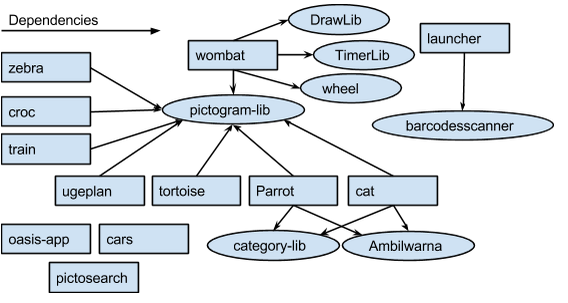
\includegraphics[width=0.8 \textwidth]{pictures/AppLibependencies.png}
	\caption{Graph of library dependencies for apps}
	\label{AppLibependencies}
\end{figure}


\subsection{Cross library dependency}
After having made all the library dependencies for the apps we did the same procedure for the libraries to find out which libraries where dependent on which library. As with the apps we started by looking at the build gradle files for the libraries, and then made a list of the dependencies, which can be seen in the list below.

\begin{table}[H]
	\centering
	\begin{tabularx}{\textwidth}{>{\raggedright}Xp{0.75\textwidth}p{0.25\textwidth}}
		\textbf{Libs} & \textbf{Dependencies}\\ \hline \noalign{\vskip 2mm}
		
		giraf-component & → dblib, local-db\\ \noalign{\vskip 2mm}
		
		dblib & → local-db\\ \noalign{\vskip 2mm}
		
		pictogram-lib & → giraf-component, dblib, local-db\\ \noalign{\vskip 2mm}
		
		sequence-viewer & → giraf-component, dblib, local-db, pictogram-lib\\ \noalign{\vskip 2mm}
		
		local-db & → metadata\\ \noalign{\vskip 2mm}
		
		category-lib  & → giraf-component, dblib, local-db, pictogram-lib\\ \noalign{\vskip 2mm}
		
		Drawlib & → NULL\\ \noalign{\vskip 2mm}
		
		TimerLib & → NULL\\ \noalign{\vskip 2mm}
		
		Ambilwarna & → NULL\\ \noalign{\vskip 2mm}
		
		barcodescanner & → NULL\\ \noalign{\vskip 2mm}
		
		wheel & → NULL\\ \noalign{\vskip 2mm}
		
		metadata & → NULL\\
		
	\end{tabularx}
	\label{Table_dependencies_liblib}
	\caption{List of cross library dependencies}
\end{table}

As with apps/library dependencies we also made a graph for cross dependency between the libraries shown in Figure \ref{LibLibdependencies}. As in the last graph the ovals are libraries and the arrows signifies dependencies. In this graph we decided to show all dependencies since there was no dependency that was the same for all libraries and because the number of dependencies was low enough, to be able to show it all without having to many lines crossing each other to be able to read the graph.


\begin{figure}[H]
	\centering
	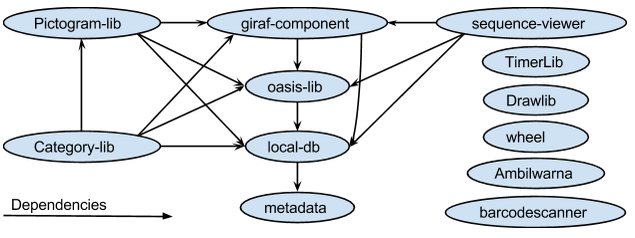
\includegraphics[width=0.8 \textwidth]{pictures/LibLibdependencies.png}
	\caption{Graph of cross library dependencies}
	\label{LibLibdependencies}
\end{figure}


\subsection{Cross App dependencies}
As the last step in finding the different dependencies we found the dependencies between the different apps. We did this in two ways, skimming through the code for any calls to another app, and by trying to run the apps on a tablet and testing if any of the apps  stopped working if another app was not installed. From the dependencies we made a graph which is shown below in Figure \ref{AppAppdependencies}. Like on the other graphs the Squares are apps and the arrows signifies dependencies, but in addition this graph also have dotted and red lines. The doted lines signifies that the app is not directly dependent, but instead dependent through another app and the red lines are dependencies we are uncertain about.

\begin{figure}[H]
	\centering
	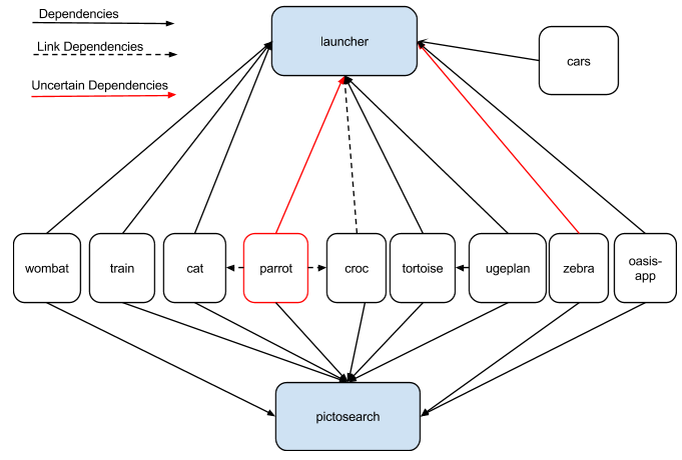
\includegraphics[width=0.8 \textwidth]{pictures/AppAppdependencies.png}
	\caption{Graph of cross app dependencies}
	\label{AppAppdependencies}
\end{figure}